
%----------------------------------------------------------------------------------------
%	IMPLEMENTAZIONE
%----------------------------------------------------------------------------------------

\section{Implementazione}\label{sec:implementazione}


\subsection{User Domain}

Per quanto riguarda l'implementazione dell'applicazione con cui si interfaccia l'utente,
è stato deciso di utilizzare il framework Svelte. \\

Questa scelta è stata dettata da un'approfondita analisi delle opzioni disponibili e
da diverse considerazioni chiave che hanno guidato questa decisione.

\subsubsection{Svelte: Leggerezza e Performance}

Svelte è emerso come la scelta ideale per l'implementazione dell'interfaccia utente.
La sua caratteristica distintiva è la mancanza di un Virtual DOM \cite{dom}, a differenza di
framework concorrenti come React \cite{react} o Vue \cite{vue}. Invece, Svelte utilizza un compilatore che
traduce il codice scritto in JavaScript, HTML \cite{html} e CSS \cite{css} direttamente in codice JavaScript
nativo altamente ottimizzato.\\

Questo si traduce in un'applicazione con un codice molto più
leggero e una maggiore velocità rispetto ad altri framework. La leggerezza è essenziale per
garantire un'esperienza utente fluida, soprattutto su dispositivi con risorse limitate.

\subsubsection{Semplicità e Velocità di Sviluppo}

Oltre alla performance, Svelte offre una curva di apprendimento molto meno ripida
rispetto ad altri framework. La sua sintassi dichiarativa e la facilità con cui è
possibile definire componenti rendono la scrittura del codice più efficiente.
Un aspetto chiave è il sistema di "store" di Svelte.\\

Nel codice fornito, notiamo l'uso dei moduli `writable` e `createEventDispatcher` per
creare e gestire uno store denominato "Stations".\\

Questo store è fondamentale per la gestione dello stato delle stazioni di ricarica
all'interno dell'applicazione. Le funzioni come `fetchStations`, `charge` e `reserve` operano
su questo store per mantenere una visione coerente e reattiva dei dati in tutta l'applicazione.

\subsubsection{Integrazione con Altre Tecnologie}

L'integrazione è stata un altro punto cruciale nella scelta di Svelte. Ad esempio,
l'applicazione utilizza Leaflet \cite{leaflet}, una libreria JavaScript per la creazione
di mappe interattive. \\

L'integrazione di Leaflet con Svelte è stata fluida, consentendo la visualizzazione
delle stazioni di ricarica sulla mappa in modo efficace ed efficiente. Inoltre,
l'applicazione è scritta in TypeScript \cite{typescript}, un linguaggio che aggiunge
tipizzazione statica a JavaScript. Questo migliora la manutenibilità del codice e aiuta
a prevenire errori comuni durante lo sviluppo.

\subsection{Auth Server}

Tra le funzionalità dell'applicazione, troviamo la possibilità di effettuare la registrazione
personale ed il login. Per gestire queste funzionalità è stato utilizzato il framework Express.js,
che offre una solida base per la creazione di un server web in Node.js. Le motivazioni dietro
questa scelta sono state ponderate attentamente.

\subsubsection{Express.js: Facilità d'Uso e Configurabilità}

Express.js è noto per la sua facilità d'uso nella creazione di server web. La sua
flessibilità lo rende una scelta eccellente per gestire le route, le richieste HTTP e
le risposte nell'applicazione. Inoltre, è stato configurato per gestire le opzioni CORS \cite{cors}
(Cross-Origin Resource Sharing), il che consente di consentire o limitare l'accesso ai
servizi del server da parte di domini esterni. Questo è fondamentale per garantire una
comunicazione sicura tra il frontend e il backend.

\subsubsection{Memorizzazione dei Dati Utente con MongoDB}

Per memorizzare i dati degli utenti, è stata fatta una scelta significativa nell'adozione
di MongoDB, un database non relazionale orientato ai documenti. Questa decisione è
stata guidata da diverse considerazioni fondamentali.

\subsubsection{Flessibilità Strutturale}

Innanzitutto, MongoDB offre una flessibilità strutturale significativa. Ciò significa
che è possibile gestire dati eterogenei senza la necessità di un rigoroso schema fisso.
Questo si è rivelato particolarmente utile durante lo sviluppo, consentendo di adattarsi
facilmente alle esigenze cambianti dell'applicazione.

\subsubsection{Scalabilità Orizzontale}

In secondo luogo, MongoDB è noto per la sua scalabilità orizzontale. Questa caratteristica
è cruciale quando si gestiscono grandi volumi di dati e carichi di traffico in crescita.
L'architettura di MongoDB consente di aggiungere nuovi nodi al cluster in modo relativamente
semplice, consentendo all'applicazione di crescere in modo fluido con il suo successo.

\subsubsection{Velocità di Sviluppo e Integrazione con JavaScript}

Infine, MongoDB si è dimostrato un'ottima scelta per accelerare lo sviluppo. La sua capacità
di memorizzare e recuperare dati in un formato JSON-like si integra perfettamente con il mondo
JavaScript, garantendo coerenza tra il modello dati del backend e quello del frontend.


\subsection{Charging Station Domain}
Per quanto riguarda l'implementazione delle componenti del Charging Station Domain, vista
la scelta fatta di progettare i sotto-componenti del dominio attraverso il modello ad attori,
la scelta su come implementarli è
ricaduta sul framework Akka.\\

Akka è un toolkit open-source per la creazione di applicazioni concorrenti e distribuite
basate sul modello ad attori. Il framework è scritto in Scala, ma è possibile utilizzarlo
anche con Java, tuttavia in questa sede si è preferito utilizzare il linguaggio Scala poichè
più flessibile, conciso e potente della controparte Java, oltre al fatto che offre un'esperienza
di sviluppo migliore col framework Akka.\\

In particolare, è stata scelta l'api \textbf{Akka Typed}, che permette di definire
gli attori attraverso un sistema di tipi, rendendo più semplice la gestione degli stessi.\\

Gli attori implementati in Akka sono stati i seguenti:
\begin{itemize}
      \item Charging Station Actor
      \item Charging Station Provider
      \item Charging Station Service
\end{itemize}

Per ognuno di essi, l'implementazione ha seguito il seguente schema:\\

\paragraph{Definizione dei messaggi scambiati tra gli attori}:
In Akka Typed, l'attore è rappresentato dal concetto di \textbf{Behavior$<T>$}, che è
un'astrazione che rappresenta il ciclo di vita di un attore. In particolare, un Behavior
è un'interfaccia funzionale che prende in input un messaggio di tipo T e restituisce un nuovo Behavior.\\

Il primo passo è stato dunque quello di definire i messaggi scambiati tra gli attori, ovvero i tipi T.\\

Per prima cosa, per ogni attore è stato definito un sealed trait base \textbf{Request} da estendere
per ogni diverso messaggio che l'attore può ricevere.\\

Dopodichè, con l'aiuto degli schemi fatti in fase di progettazione, sono state create,
per ogni attore, diverse case classes le quali estendono Request e rappresentano i diversi
messaggi specifici che l'attore può ricevere.\\

Segue un esempio di definizione dei messaggi per l'attore Charging Station Actor:
\begin{lstlisting}[language=scala]
object ChargingStationEvents:
      sealed trait Request
      case class AskState(replyTo: ActorRef[ChargingStationProvider.Request]) extends Request
      case class Charge(request: ChargeRequest, replyTo: ActorRef[ChargeRequestResult]) extends Request
      case class Reserve(reservation: Reservation, replyTo: ActorRef[ReservationResult]) extends Request
      case class StopCharge() extends Request
\end{lstlisting}

\paragraph{Definizione delle reazioni ai messaggi}:
Come anticipato, il Behavior$<T>$ è un'interfaccia funzionale che prende in input un
messaggio di tipo T e restituisce un nuovo Behavior.\\

Dunque, per completare l'implementazione di un attore è necessario fornire un implementazione
coerente di Behavior$<T>$. A tale scopo, Akka fornisce svariate funzioni di factory racchiuse
nell'object \textbf{Behaviors}, che permettono di creare Behavior$<T>$ in modo semplice e conciso.\\

A seconda della complessità dell'attore da implementare, sono state utilizzate le seguenti
funzioni di factory:
\begin{itemize}
      \item \textbf{Behaviors.receive}: questa funzione permette di creare un Behavior$<T>$
            che reagisce a un messaggio di tipo T. In particolare, prende in input una funzione
            che prende in input il messaggio di tipo T e l'\textbf{Actor Context} e restituisce
            un Behavior$<T>$.\\

            L'Actor Context è un elemento chiave del framework Akka, poichè permette all'attore
            di manipolare od ottenere informazioni circa il suo contesto di esecuzione.
            Questo oggetto è necessario laddove un attore debba spawnare un attore figlio,
            accedere al proprio riferimento univoco, o utilizzare funzionalità di logging.\\

            Questa factory è stata utilizzata per implementare Charging Station Actor e Charging
            Station Provider.
      \item \textbf{Behaviors.receiveMessage}: questa funzione permette di creare un Behavior$<T>$
            che reagisce a un messaggio di tipo T. In particolare, prende in input una funzione che
            prende in input il messaggio di tipo T e restituisce un Behavior$<T>$.\\

            È una versione più concisa della receive classica poichè non necessita dell'Actor
            Context. Questa factory è stata utilizzata per implementare Charging Station Service.
      \item \textbf{Behaviors.setup}: questa funzione non reagisce a nessun messaggio, ma permette
            di eseguire del codice una volta che l'attore è stato spawnato. In particolare, prende in
            input una funzione che prende in input l'Actor Context e restituisce un Behavior$<T>$.\\

            Questa factory è stata utilizzata per implementare Charging Station Actor e Charging
            Station Provider.
\end{itemize}

Di seguito un esempio semplificato di implementazione di un attore utilizzando Behaviors.setup e
Behaviors.receive:\\

\newpage

\begin{lstlisting}[language=scala]
object ChargingStationProvider:
      def apply(): Behavior[ChargingStationProvider.Request] = 
            Behaviors setup { context =>
                  // esegui operazioni preliminari dipendenti dall'Actor Context
                  running() // separiamo il codice del setup da eseguire una sola volta con il codice effettivo del Behavior
            }
      private def running(): Behavior[ChargingStationProvider.Request] = 
            Behaviors receive { (context, message) =>
                  // reagisci al messaggio
                  running() // ritorna ricorsivamente questo Behavior
            }
\end{lstlisting}

\subsubsection{Creazione di un cluster di attori}
Nella visione classica di Akka, uno o più attori eseguono concorrentemente all'interno dello stesso
\textbf{Actor System}.\\

L'Actor System è un'astrazione che rappresenta un ambiente di esecuzione per tutti gli attori.
In particolare, è responsabile di allocare le risorse necessarie per l'esecuzione degli attori,
come ad esempio i thread.
L'Actor System è dunque una struttura molto pesante e costosa in termini computazionali, e dovrebbe
esistere un solo Actor System per applicazione.
Esso rappresenta dunque uno o più attori che comunicano tra loro ed eseguono concorrentemente all'interno
di un unico processo e, quindi, dispositivo fisico.\\

Come si può facilmente intuire, questa visione di Akka non è adatta per la realizzazione di un sistema
distribuito, poichè non permette di eseguire attori di uno stesso Actor System su dispositivi fisici
diversi. È necessario dunque riuscire ad eseguire ogni attore logicamente indipendente in un
proprio Actor System, e far comunicar e tra loro gli attori di diversi Actor System.\\

A tal scopo, Akka fornisce il modulo \textbf{Akka Cluster}\cite{akkacluster}, che permette
di creare un cluster di Actor Systems che comunicano tra loro attraverso la rete.\\

Dal punto di vista dello sviluppatore, questo modulo è estremamente potente, poichè permette,
con minima aggiunta di codice, di creare un cluster di attori che comunicano tra loro anche se
appartenenti a dispositivi fisici diversi.\\

Uno degli elementi chiave dell'api di Akka cluster è il \textbf{Receptionist}, che è responsabile
di registrare gli attori all'interno del cluster e di fornire un riferimento ad essi.\\

Un attore dunque partecipa al cluster esponendo una \textbf{ServiceKey}, che utilizza per registrarsi
al cluster tramite Receptionist. Una volta registrato, l'attore può essere scoperto dagli attori che
si registrano alla sua ServiceKey sempre tramite Receptionist.\\

Il Receptionist, al momento della registrazione di un nuovo attore tramite ServiceKey, notifica
tutti gli attori sottoscritti a quella ServiceKey con il nuovo set di attori registrati.\\

Questo comportamento è riassunto nel seguente diagramma di sequenza \ref{fig:cluster}:

\begin{figure}[H]
      \centering
      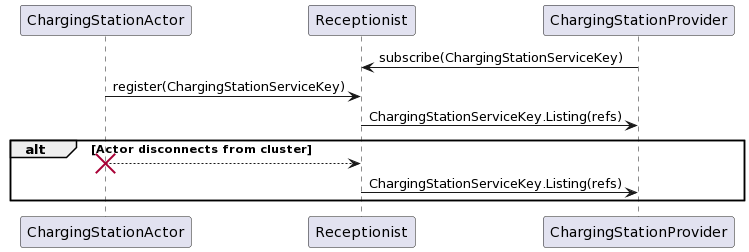
\includegraphics[width=0.8\textwidth]{images/cluster.png}
      \caption{Diagramma di sequenza che mostra il comportamento del Receptionist}
      \label{fig:cluster}
\end{figure}

\subsubsection{Serializzazione intra cluster}
Per permettere la comunicazione tra attori di diversi Actor System, è necessario
che i messaggi scambiati tra di essi siano serializzabili. Per raggiungere questo scopo abbiamo
adottato la libreria \textbf{akka-serialization-jackson} \cite{akkaserjack}, che permette di serializzare oggetti
in vari formati definendo dei \textbf{SerializationBindings}. In questo caso abbiamo utilizzato
jackson-cbor.

\subsubsection{Esposizione di un servizio REST}
Per esporre un servizion REST basato sul protocollo HTTP, abbiamo utilizzato il modulo \textbf{Akka HTTP},
che permette di creare un server HTTP in modo semplice e conciso.\\

In particolare, l'attore Charging Station Service all'interno del suo setup esegue le seguenti operazioni:
\begin{itemize}
      \item Definisce le routes ed i rispettivi handlers attraverso il DSL \textbf{Server Directives} di Akka HTTP.
      \item Esegue il binding del server HTTP ad un indirizzo IP e porta specificati.
      \item Restituisce un Behavior che risponde ad un messaggio di Stop, causando l'unbinding del server HTTP e la terminazione del servizio e dell'attore stesso.
\end{itemize}

\subsubsection{Marshalling ed Unmarshalling}
Per la conversione dei bodies delle richieste HTTP in oggetti Scala e viceversa, abbiamo utilizzato
il modulo \textbf{Spray Json}, che permette di definire dei \textbf{RootJsonFormat} per i tipi di dato
del modello per i quali vogliamo che vengano eseguiti Marshalling ed Unmarshalling automatici.\\

\subsection{Tecnologie impiegate}

In questa sezione, verranno presentate in dettaglio le principali tecnologie utilizzate per implementare
il sistema e le motivazioni che ci hanno spinto a sceglierle.

\subsubsection{Applicazione utente}

Per l'implementazione dell'applicazione utente, sono state impiegate diverse tecnologie chiave:

\begin{itemize}
      \item \textbf{Svelte}: Svelte è il framework front-end principale utilizzato per la creazione
            dell'interfaccia utente dell'applicazione. La sua caratteristica distintiva è la compilazione
            del codice Svelte in JavaScript altamente ottimizzato. Questo framework permette di scrivere
            codice dichiarativo che si traduce in un'applicazione web reattiva ed efficiente.

      \item \textbf{Svelte Kit} \cite{sveltekit}: Svelte Kit è una libreria aggiuntiva che semplifica la gestione
            delle route e delle pagine in un'applicazione Svelte. Questo è fondamentale per creare un'applicazione
            a pagine multiple in modo strutturato e organizzato.

      \item \textbf{Leaflet}: Leaflet è una libreria JavaScript utilizzata per creare mappe interattive.
            È stata impiegata nell'applicazione per l'integrazione delle mappe e la visualizzazione delle
            stazioni di ricarica per veicoli elettrici.

      \item \textbf{TypeScript}: TypeScript è un linguaggio di programmazione che aggiunge tipizzazione
            statica a JavaScript. Questo miglioramento della tipizzazione rende il codice più affidabile e
            agevola la manutenzione.

      \item \textbf{Vite} \cite{vite}: Vite è un bundler e un task runner veloce progettato per lo sviluppo
            front-end. Grazie al suo sistema di moduli nativo e alla ricarica a caldo, semplifica
            notevolmente lo sviluppo e l'ottimizzazione del codice.

      \item \textbf{Svelte Geolocation} \cite{sveltegeo}: La dipendenza "svelte-geolocation" è stata utilizzata per
            accedere alla funzionalità di geolocalizzazione del dispositivo all'interno dell'applicazione.
            Questo è utile per determinare la posizione dell'utente e fornire informazioni basate sulla
            sua posizione, ad esempio la visualizzazione delle stazioni di ricarica più vicine.

      \item \textbf{Svelte QR Scanner} \cite{scanner}: "Svelte-qr-scanner" è stato integrato nell'applicazione per
            consentire la scansione dei codici QR. Questa funzionalità è utilizzata per diverse finalità,
            ad esempio la lettura di QR code per lo sblocco di una colonnina ed il conseguente inizio della
            ricarica.
\end{itemize}

\subsubsection{Authentication server}

Per quanto riguarda il server utilizzato per l'autenticazione, sono state utilizzate le seguenti tecnologie:

\begin{itemize}
      \item \textbf{Express.js}: Express è un framework web per Node.js che semplifica
            la creazione di server web. È utilizzato per gestire le route, le richieste HTTP e
            le risposte nell'applicazione.

      \item \textbf{MongoDB}: MongoDB è un database non relazionale orientato ai documenti.
            È utilizzato per memorizzare i dati dell'applicazione in formato JSON-like. La scelta di
            MongoDB è stata motivata dalla flessibilità strutturale, dalla scalabilità orizzontale e
            dalla facilità di sviluppo.

      \item \textbf{Mongoose} \cite{mongoose}: Mongoose è una libreria Node.js che semplifica l'interazione con
            il database MongoDB. È utilizzato per definire gli schemi dei dati e per eseguire operazioni
            di query nel database in modo più intuitivo.

      \item \textbf{bcrypt} \cite{bcrypt}: bcrypt è una libreria per la crittografia delle password. È utilizzata
            per proteggere le password degli utenti nel database, garantendo che siano memorizzate in modo sicuro.

      \item \textbf{CORS}: CORS (Cross-Origin Resource Sharing) è una tecnologia che consente di
            gestire le richieste HTTP provenienti da origini diverse. È utilizzata per consentire o
            limitare l'accesso ai servizi del server da parte di domini esterni.

      \item \textbf{dotenv} \cite{dotenv}: dotenv è un modulo che permette di caricare variabili d'ambiente da
            un file di configurazione. È utilizzato per gestire le variabili d'ambiente nell'applicazione,
            consentendo la configurazione di parametri sensibili come le chiavi segrete.

      \item \textbf{jsonwebtoken} \cite{jsonwebtoken}: jsonwebtoken è una libreria per la gestione dei JSON Web Token (JWT).
            È utilizzata per l'autenticazione e l'autorizzazione degli utenti nell'applicazione.
\end{itemize}

\paragraph{Perchè MongoDB}

Le scelte che hanno portato alla decisione dell'utilizzo di MongoDB anzichè
di un database relazionale sono state le seguenti:

\begin{itemize}
      \item \textbf{Flessibilità nella struttura dei dati}: MongoDB consente di gestire

            dati eterogenei senza la necessità di uno schema fisso.

      \item \textbf{Scalabilità orizzontale}: La capacità di scalare orizzontalmente è
            cruciale per gestire grandi volumi di dati e carichi di traffico crescenti.

      \item \textbf{Velocità di sviluppo}: MongoDB semplifica lo sviluppo rapido,
            consentendo di memorizzare e recuperare dati in formato JSON-like.

      \item \textbf{Integrazione nativa con JavaScript}: Si integra bene con applicazioni
            JavaScript, fornendo coerenza tra il modello dati del backend e quello del frontend.
\end{itemize}




% \subsection{User App - A}

% %Considerazioni generali sulle particolarità di svelte

% Per quanto riguarda l'implementazione dell'applicazione con cui si interfaccia l'utente,
% è stato deciso di utilizzare il framework Svelte. Questa scelta è stata dettata dal fatto
% che Svelte è un framework molto leggero, che non utilizza un Virtual DOM, ma che si basa
% su un compilatore che traduce il codice scritto in Javascript, HTML e CSS in codice Javascript
% nativo. Questo permette di avere un codice molto più leggero e veloce rispetto ad altri
% framework come React o Vue. Inoltre, Svelte è molto semplice da utilizzare e permette
% di creare applicazioni web in modo molto intuitivo e veloce.


% \subsubsection{Svelte store}
% Lo "store" in Svelte è un meccanismo per gestire lo stato dell'applicazione in modo reattivo e condiviso tra le diverse parti dell'applicazione. Nella porzione di codice fornita, vengono utilizzati i moduli \texttt{writable} e \texttt{createEventDispatcher} per creare e gestire uno store denominato "Stations". Ecco una breve descrizione di ciò che viene fatto nel codice:
% \begin{enumerate}[label=\arabic*.]
%       \item \textbf{Creazione dello Store "Stations"}: La riga
%             \texttt{export const Stations = writable([])} inizializza uno store
%             Svelte chiamato "Stations" utilizzando la funzione \texttt{writable}.
%             Questo store sarà utilizzato per memorizzare e condividere un elenco
%             di stazioni di ricarica all'interno dell'applicazione.

%       \item \textbf{Definizione di Funzioni per Interagire con lo Store}:
%             \begin{enumerate}[label=\arabic{enumi}.\arabic*]
%                   \item \textit{fetchStations}: Questa funzione effettua una richiesta
%                         HTTP per recuperare l'elenco delle stazioni di ricarica dal server (AKKA SERVER)
%                         e poi lo trasforma in un formato appropriato. Infine, aggiorna il valore dello
%                         store "Stations" utilizzando \textit{Stations.set(newStations)}. In questo modo,
%                         l'elenco delle stazioni è disponibile globalmente all'interno dell'applicazione.

%                   \item \texttt{charge}: Questa funzione invia una richiesta HTTP al server AKKA per avviare una sessione di ricarica per un utente presso una stazione di ricarica specifica. Se l'operazione ha successo, l'applicazione viene reindirizzata alla pagina principale.

%                   \item \texttt{reserve}: Simile a \texttt{charge}, questa funzione invia una richiesta HTTP per prenotare una stazione di ricarica e reindirizza l'applicazione alla pagina principale se ha successo.
%                   \item \textit{addFavourite}: Questa funzione invia una
%                         richiesta HTTP al server (EXPRESS SERVER) per aggiungere una stazione
%                         di ricarica ai preferiti di un utente. Se la richiesta ha successo, viene
%                         generato un evento personalizzato per notificare altre parti dell'applicazione.

%                   \item \texttt{removeFavourite}: Simile a \texttt{addFavourite}, questa funzione invia una richiesta HTTP per rimuovere una stazione dai preferiti di un utente e genera un evento se l'operazione ha successo.
%             \end{enumerate}
% \end{enumerate}


% \subsection{Auth Server}

% % parlare di express e nodejs e mongodb

% Tra le funzionalità dell'applicazione, troviamo la possibilità di effettuare la
% registrazione personale ed il login. Per gestire queste funzionalità è stato utilizzato
% il framework Express.js, che permette di creare un server web in Node.js e include
% la configurazione delle opzioni CORS per consentire richieste da qualsiasi origine.
% Inoltre, per memorizzare i dati degli utenti, è stato utilizzato MongoDB,
% un database non relazionale che permette di memorizzare i dati in formato JSON.
% Per interfacciarsi con il database, è stato utilizzato il modulo Mongoose, che
% permette di definire degli schemi per i dati che vengono memorizzati nel database.


% \subsection{Tecnologie impiegate - A}

% In questa sezione verranno presentate le principali tecnologie utilizzate per implementare il sistema e le motivazioni che ci hanno spinto a sceglierle.

% \subsubsection{Applicazione utente}
% Le tecnologie principali utilizzate per l'implementazione dell'applicazione utente sono:

% \begin{itemize}
%       \item \textbf{Svelte}: Svelte è il framework front-end principale utilizzato per la creazione
%             dell'interfaccia utente dell'applicazione. La sua caratteristica distintiva è la compilazione
%             del codice Svelte in JavaScript altamente ottimizzato. Questo framework permette di scrivere
%             codice dichiarativo che si traduce in un'applicazione web reattiva ed efficiente.

%       \item \textbf{Svelte Kit}: Svelte Kit è una libreria aggiuntiva che semplifica la gestione
%             delle route e delle pagine in un'applicazione Svelte. Questo è fondamentale per creare
%             un'applicazione a pagine multiple in modo strutturato e organizzato.

%       \item \textbf{Leaflet}: Leaflet è una libreria JavaScript utilizzata per creare mappe
%             interattive. È stata impiegata nell'applicazione per l'integrazione delle mappe e la
%             visualizzazione delle stazioni di ricarica per veicoli elettrici.

%       \item \textbf{TypeScript}: TypeScript è un linguaggio di programmazione che aggiunge
%             tipizzazione statica a JavaScript. Questo miglioramento della tipizzazione rende
%             il codice più affidabile e agevola la manutenzione.

%       \item \textbf{Vite}: Vite è un bundler e un task runner veloce progettato per lo
%             sviluppo front-end. Grazie al suo sistema di moduli nativo e alla ricarica a caldo,
%             semplifica notevolmente lo sviluppo e l'ottimizzazione del codice.

%       \item \textbf{Svelte Geolocation}: La dipendenza "svelte-geolocation" è stata utilizzata
%             per accedere alla funzionalità di geolocalizzazione del dispositivo all'interno
%             dell'applicazione. Questo è utile per determinare la posizione dell'utente e fornire
%             informazioni basate sulla sua posizione, ad esempio la visualizzazione delle stazioni di ricarica
%             più vicine.

%       \item \textbf{Svelte QR Scanner}: "Svelte-qr-scanner" è stato integrato nell'applicazione
%             per consentire la scansione dei codici QR. Questa funzionalità è utilizzata per diverse
%             finalità, ad esempio la lettura di QR code per lo sblocco di una colonnina ed il
%             conseguente inizio della ricarica.
% \end{itemize}

% \subsubsection{Authentication server}

% Per quanto riguarda il server utilizzato per l'autenticazione sono state utilizzate le seguenti tecnologie:

% \begin{itemize}

%       \item \textbf{express}: Express è un framework web per Node.js che semplifica
%             la creazione di server web. È utilizzato per gestire le route, le richieste
%             HTTP e le risposte nell'applicazione.

%       \item \textbf{mongodb}: MongoDB è un database non relazionale orientato ai
%             documenti. È utilizzato per memorizzare i dati dell'applicazione in formato
%             JSON-like. MongoDB è una scelta comune per applicazioni che richiedono scalabilità
%             e flessibilità nella gestione dei dati.

%       \item \textbf{mongoose}: Mongoose è una libreria Node.js che semplifica l'interazione
%             con il database MongoDB. È utilizzato per definire gli schemi dei dati e per
%             eseguire operazioni di query nel database in modo più intuitivo.

%       \item \textbf{bcrypt}: bcrypt è una libreria per la crittografia delle password.
%             È utilizzata per proteggere le password degli utenti nel database, garantendo che
%             siano memorizzate in modo sicuro.

%       \item \textbf{cors}: CORS (Cross-Origin Resource Sharing) è una tecnologia che
%             consente di gestire le richieste HTTP provenienti da origini diverse. È utilizzata
%             per consentire o limitare l'accesso ai servizi del server da parte di domini esterni.

%       \item \textbf{dotenv}: dotenv è un modulo che permette di caricare variabili
%             d'ambiente da un file di configurazione. È utilizzato per gestire le variabili
%             d'ambiente nell'applicazione, consentendo la configurazione di parametri
%             sensibili come le chiavi segrete.

%       \item \textbf{jsonwebtoken}: jsonwebtoken è una libreria per la gestione dei
%             JSON Web Token (JWT). È utilizzata per l'autenticazione e l'autorizzazione
%             degli utenti nell'applicazione.

% \end{itemize}

% Le scelte che hanno portato alla decisione dell'utilizzo di MongoDB anzichè
% di un database relazionale sono state le seguenti:

% \begin{itemize}
%       \item \textbf{Flessibilità nella struttura dei dati}: MongoDB consente di gestire

%             dati eterogenei senza la necessità di uno schema fisso.

%       \item \textbf{Scalabilità orizzontale}: La capacità di scalare orizzontalmente è
%             cruciale per gestire grandi volumi di dati e carichi di traffico crescenti.

%       \item \textbf{Velocità di sviluppo}: MongoDB semplifica lo sviluppo rapido,
%             consentendo di memorizzare e recuperare dati in formato JSON-like.

%       \item \textbf{Integrazione nativa con JavaScript}: Si integra bene con applicazioni
%             JavaScript, fornendo coerenza tra il modello dati del backend e quello del frontend.
% \end{itemize}



%Esporre i principali problemi affrontati durante l'effettiva realizzazione delle componenti hardware/software e illustrare le soluzioni implementative adottate. Se l'elaborato ha previsto l'utilizzo di tecnologie già disponibili sul mercato, discuterne brevemente le caratteristiche e motivarne l'adozione rispetto ad altre soluzioni assimilabili.\\

%\textbf{NOTA: in questa sezione devono essere riportate esclusivamente le porzioni di codice ritenute particolarmente significative. Il codice sorgente nella sua interezza, opportunamente commentato, deve essere consegnato separatamente dalla relazione in un archivio compresso.}\\


%Vincoli circa la lunghezza della sezione (escluse didascalie, tabelle, testo nelle immagini, schemi):

%\vspace{1cm}
%\begin{tabular}{l|rr}
%                 & Numero minimo di battute & Numero massimo di battute \\
%    \hline
%    1 componente & 5000                     & 11000                     \\
%    2 componenti & 8000                     & 16000                     \\
%    3 componenti & 10000                    & 21000                     \\
%    \hline
%\end{tabular}


\newpage